\documentclass[pdftex,spanish]{pucthesis}

\usepackage{graphicx}
\usepackage{float}
\usepackage{subfigure}
\usepackage[table]{xcolor}
\usepackage{amsmath}
\counterwithout{figure}{chapter}
\usepackage{amsfonts}
\usepackage{amssymb}
\usepackage{booktabs}
\usepackage{multirow}
\usepackage{etoolbox}
\apptocmd{\sloppy}{\hbadness 10000\relax}{}{}
\usepackage[hidelinks,pdfusetitle,pdfdisplaydoctitle]{hyperref}
\usepackage[notocbib]{apacite}
\usepackage{doi}
\renewcommand{\doitext}{}

\makeatletter
\renewcommand{\normalsize}{%
  \@setfontsize\normalsize\@xipt{13.6}%
  \abovedisplayskip 11\p@ \@plus3\p@ \@minus6\p@
  \abovedisplayshortskip \z@ \@plus3\p@
  \belowdisplayshortskip 6.5\p@ \@plus3.5\p@ \@minus3\p@
  \belowdisplayskip \abovedisplayskip
  \let\@listi\@listI}
\normalsize
\makeatother

\begin{document}
\raggedbottom

\setstretch{1.4}
\mdate{Octubre 2026}
\version{2}

\title[PLANIFICACI\'ON DE LA OPERACI\'ON DE LOS BUSES EL\'ECTRICOS\\ EN LA RED METROPOLITANA DE MOVILIDAD DE SANTIAGO\\ GRUPO 24]
   {\bf PLANIFICACI\'ON DE LA OPERACI\'ON DE LOS BUSES EL\'ECTRICOS\\ EN LA RED METROPOLITANA DE MOVILIDAD DE SANTIAGO\\ GRUPO 24}
\author[Integrantes:]{Integrantes:\\
\textnormal{\small{
Nicol\'as Bennett\\
Antonio De Frutos\\
Claudio Hasb\'un\\
Agust\'in Irarr\'azaval\\
Joaqu\'in Jim\'enez\\
Alonso Muelas}
}}

\address{Escuela de Ingenier\'ia\\
                   Pontificia Universidad Cat\'olica de Chile\\
                   Vicu\~na Mackenna 4860\\
                  Santiago, Chile\\
                  {\it Tel.\/} : 56 (2) 354-2000}

\advisor{\textbf{Profesor Gu\'ia:} Agust\'in Chiu}
\ogrsmember{\textbf{Ayudante Tutor:} Max Burr}
\date{Octubre 2026}
\copyrightname{Grupo 24}
\copyrightyear{2026}

\NoChapterPageNumber
\pagenumbering{roman}
{\hfuzz=11pt\maketitle}

\pdfbookmark{\contentsname}{toc}
\tableofcontents
\listoffigures
\listoftables
\cleardoublepage

\phantomsection \label{resumen}
\chapter*{RESUMEN}
% Completar al final del proyecto: problema, objetivo, metodología, resultados
% principales y conclusión. Incluir palabras clave al final.
\noindent\textit{[Redactar un resumen autocontenido del caso, el objetivo, la
metodología seleccionada, el trabajo realizado, los resultados preliminares y
las conclusiones principales.]}

\vfill
\noindent\textbf{Palabras clave:} [Agregar entre tres y seis palabras clave.]
\cleardoublepage

\pagenumbering{arabic}

\chapter[INTRODUCCI\'ON]{Introducci\'on}
La electrificación del transporte público es una de las principales vías para reducir las emisiones y el ruido en las ciudades, y Santiago ha avanzado hasta operar una de las flotas de buses eléctricos más grandes fuera de China [citar fuente verificada]. Sin embargo, un bus eléctrico no se opera como uno diésel: su autonomía es limitada, su recarga toma tiempo y solo puede hacerse en electroterminales con pocos cargadores. Por esta razón, decidir qué bus hace cada viaje ya no basta, porque también hay que decidir cuándo y dónde carga cada bus, y ambas decisiones se condicionan entre sí.

Esa dependencia hace costosa una mala planificación, pues las horas de mayor demanda de viajes coinciden en parte con las de electricidad más cara y la recarga se concentra cuando los buses vuelven a los electroterminales. El resultado puede ser más buses de los necesarios, mayor gasto en energía y más kilómetros sin pasajeros, o incluso planes que no pueden ejecutarse porque la infraestructura no alcanza. Pero la misma complejidad abre oportunidades, ya que aprovechar mejor cada bus, por ejemplo haciéndolo atender viajes de más de una ruta, y repartir la recarga a lo largo del día puede reducir la flota, el gasto en energía y la presión sobre una infraestructura escasa y costosa de ampliar. Resolver bien este problema es, por lo tanto, una condición para que la electrificación sea sostenible desde el punto de vista económico y operacional.

Este informe continúa el Informe 1, que caracterizó el problema como un problema de asignación de vehículos eléctricos, conocido como E-VSP, y propuso una descomposición espaciotemporal con horizonte rodante. La revisión señaló que esa propuesta era demasiado compleja de implementar y pidió revisar en profundidad las estrategias de agrupamiento, por lo que esta entrega replantea la metodología y revisa distintas estrategias de agrupamiento de rutas.

En este contexto, el objetivo general es proponer y evaluar una metodología de planificación diaria de buses eléctricos que minimice el costo total de operación, y medir su desempeño frente a un caso base. Para lograrlo, se busca formular matemáticamente el problema, cuantificar el ahorro que genera permitir que un bus atienda viajes de rutas distintas, evaluar cómo la batería y los puestos de carga afectan el tamaño de la flota y el costo, estimar el valor de programar la carga frente a cargar solo cuando el bus lo necesita, e identificar los supuestos con mayor efecto sobre los resultados.

El entregable esperado es un plan operacional diario que resuelva las decisiones de asignación de buses a viajes, de traslados sin pasajeros y de recarga. Este plan se compone de las jornadas de cada bus, entendidas como la secuencia ordenada de expediciones y traslados que realiza entre su salida y su regreso al electroterminal, y de un programa de carga que especifica las ventanas de tiempo en que cada bus se recarga, el electroterminal utilizado y la energía repuesta. A esto se suma el desglose del costo total de la operación y los indicadores de desempeño calculados frente a un caso base.



\chapter[PROBLEMA, DATOS Y MODELO]{Descripci\'on del problema, datos y modelo}
\section{Descripción del problema}


La red de buses de RED organiza su servicio en rutas, la mayoría con un sentido de ida y otro de vuelta, y cada viaje se repite durante el día con una frecuencia que cambia según la hora. Los buses salen de un electroterminal, realizan uno o más viajes y regresan a él para recargarse. Un electroterminal es una instalación donde los buses se estacionan y cargan, y en cada instante solo pueden cargar tantos buses como puestos de carga tenga. Además, la electricidad no cuesta lo mismo a toda hora, sino que su precio depende del tramo horario.

En este escenario intervienen cuatro actores. El operador de la red define los viajes que deben cubrirse y busca hacerlo al menor costo. La flota aporta los buses, todos del mismo modelo. Los electroterminales ofrecen el lugar y los puestos donde esos buses pueden recargarse. Por último, el sistema eléctrico fija la tarifa de la energía según el tramo horario. Los pasajeros no se modelan como actor, y la oferta programada hace de demanda.

El problema consiste en planificar, para un día laboral tipo, de lunes a viernes, la operación de una flota homogénea de buses eléctricos BYD K9 de RED. El día incluye 64.502 viajes programados, denominados expediciones, repartidos en 417 rutas. Cada bus tiene una batería de 350 kWh, que entrega una autonomía útil de 225 km, y se recarga con una potencia de 180 kW, lo que toma unos 105 minutos entre el 10\% y el 100\%. La carga solo puede hacerse en cinco electroterminales, que en conjunto tienen 700 puestos, y cada puesto atiende un bus a la vez.

Hay tres decisiones por tomar. La primera es qué bus realiza cada expedición y en qué orden. La segunda son los traslados sin pasajeros, que incluyen salir del electroterminal hacia el primer viaje, volver al terminar y moverse entre viajes consecutivos, y que en conjunto se denominan deadhead. La tercera es la recarga, es decir, cuándo, dónde y cuánta energía recibe cada bus.

La solución debe cumplir seis reglas. Cada expedición se cubre exactamente una vez. La secuencia de cada bus debe ser posible en el tiempo, de modo que alcance a trasladarse entre un viaje y el siguiente. La batería nunca baja del 10\%. En ningún momento hay más buses cargando que puestos disponibles. Cada bus debe volver al electroterminal del que salió y cada bus termina el día con la misma batería con que lo empezó, porque al día siguiente se repite el ciclo y de otro modo se estaría usando energía que nadie repone.

Por último, el objetivo principal es minimizar el costo total de operación. Se puede ver en la siguiente ecuación:

\begin{equation}
    \min
    \left\{
        250 B + 0{,}5 K_{\mathrm{dh}} + 0{,}03 T_{\mathrm{espera}}
        + 5 N_{\mathrm{cargas}}
        + \sum_{h \in H} p_h E_h
    \right\}.\tag{1}
\end{equation}

Aquí, $B$ es el tamaño de la flota, que es irrestricto, $K_{\mathrm{dh}}$ los kilómetros recorridos sin pasajeros, $T_{\mathrm{espera}}$ los minutos de espera, $N_{\mathrm{cargas}}$ el número de eventos de carga, y $E_h$ la energía (en kWh) cargada durante el tramo horario $h$, cuyo precio es $p_h$ (entre 0,10 y 0,22 USD/kWh).



\section{Datos y preparación}
\label{sec:datos-informe2}

Los datos provienen de dos fuentes. La primera es la programación de la red de buses de RED, vigente entre julio y diciembre de 2026, que describe las rutas, los patrones de viaje con sus horarios y frecuencias, los paraderos y los trazados de cada recorrido. La segunda son los parámetros entregados por el curso, que fijan los electroterminales, las características del bus, los costos y las tarifas por tramo horario. \\
Por otra parte, se filtraron estos datos. Primero, se conservaron solo los buses de RED, excluyendo Metro, Metrotren y el bus al aeropuerto, y solo el día laboral. \\
Segundo, como los viajes se definen por frecuencia y no por horarios fijos, cada uno de los 6.620 patrones se expandió en las salidas que realiza durante el día. Un mismo patrón se repite varias veces, así que su identificador no distingue entre salidas, y por eso se asignó un identificador propio a cada expedición. Tercero, se calculó para cada expedición su distancia y su energía, esta última como la distancia por un consumo de 1,4 kWh por kilómetro. \\
Los datos no incluyen distancias de traslado sin pasajeros ni una asignación previa de viajes a buses, por lo que ambos se construyen en el modelo.

\section{Analisis de datos y hallazgos}
\label{sec:modelo-informe2}
A continuacion, se presenta un grafico que contiene informacion sobre la demanda de buses y las tarifas energeticas durante el dia:

\begin{figure}[H]
\centering
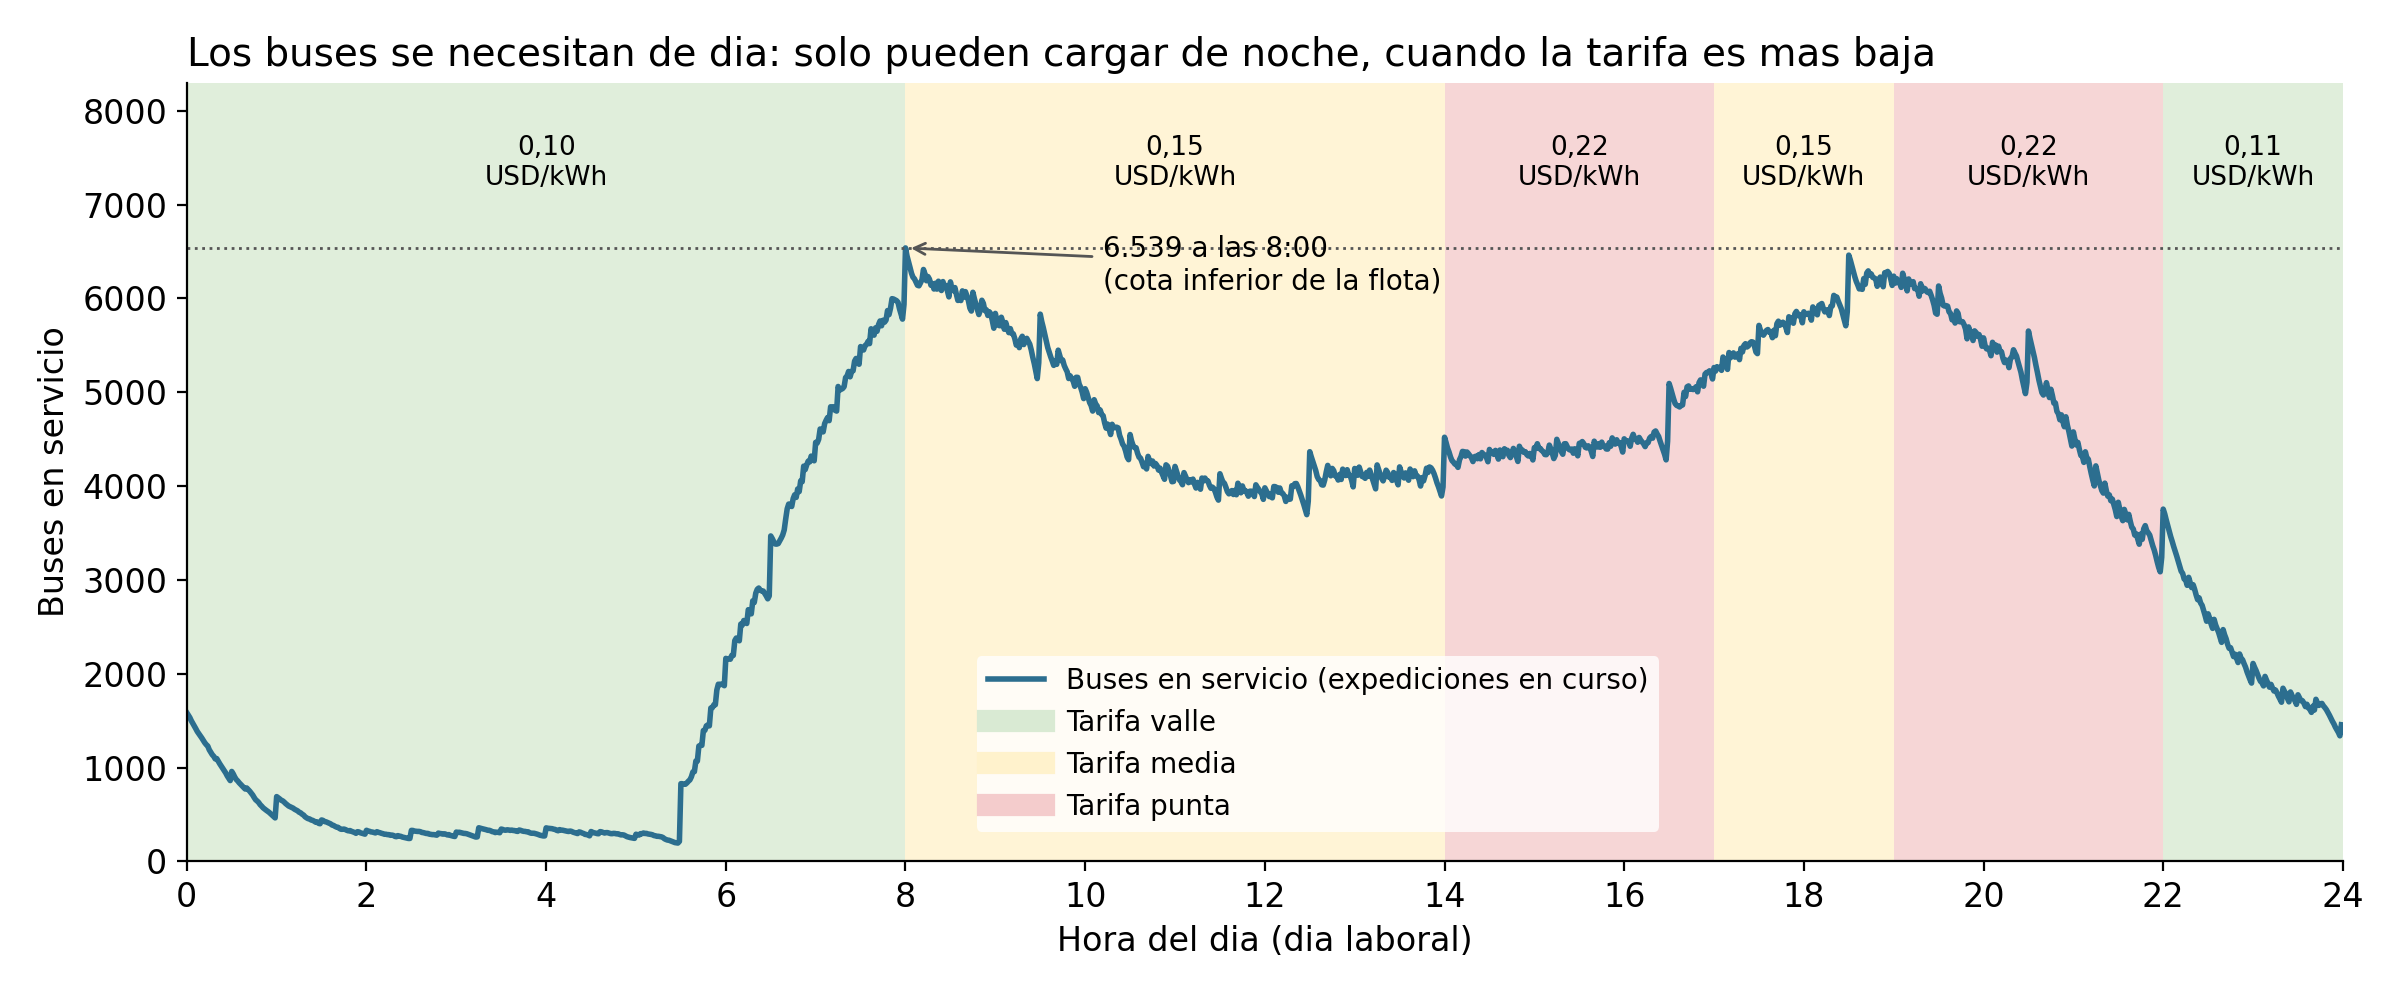
\includegraphics[width=\textwidth]{figures/G1_demanda_y_tarifa.png}
\caption{Demanda de buses y tarifas energéticas durante el día}
\label{fig:demanda-tarifa}
\end{figure}

Como se puede ver en la figura 1, la demanda de expediciones presenta 2 peaks, uno a las 8:00 con 6539 buses circulando simultaneamente, y otro a las 18:30 con 6462.Este primer peak es una cota inferior del tamaño de flota para cualquier metodologia. \\
Por otra parte,la demanda en general se concentra durante el dia por lo que logicamente las recargas se concentraran principalmente en horarios nocturnos,que justo coinciden en los tramos horarios en que las tarifas son mas baratas de 0:00 a 8:00 am y de 22:00 a 24:00, en cambio, los tramos mas caros, de 14:00 a 17:00 pm y de 19:00 a 22:00 pm, coinciden en horarios en que la demanda aun es intensa, pero no en su punto maximo.

Tambien se encontraron distintos hallazgos que condicionaron la modelacion de este problema.\\ 
De las 300 rutas cuyos dos sentidos son identificables, el 94,7\% termina la ida a menos de 500 m del punto donde comienza la vuelta, con una mediana de 85 m, como muestra la Figura 2:

\begin{figure}[H]
\centering
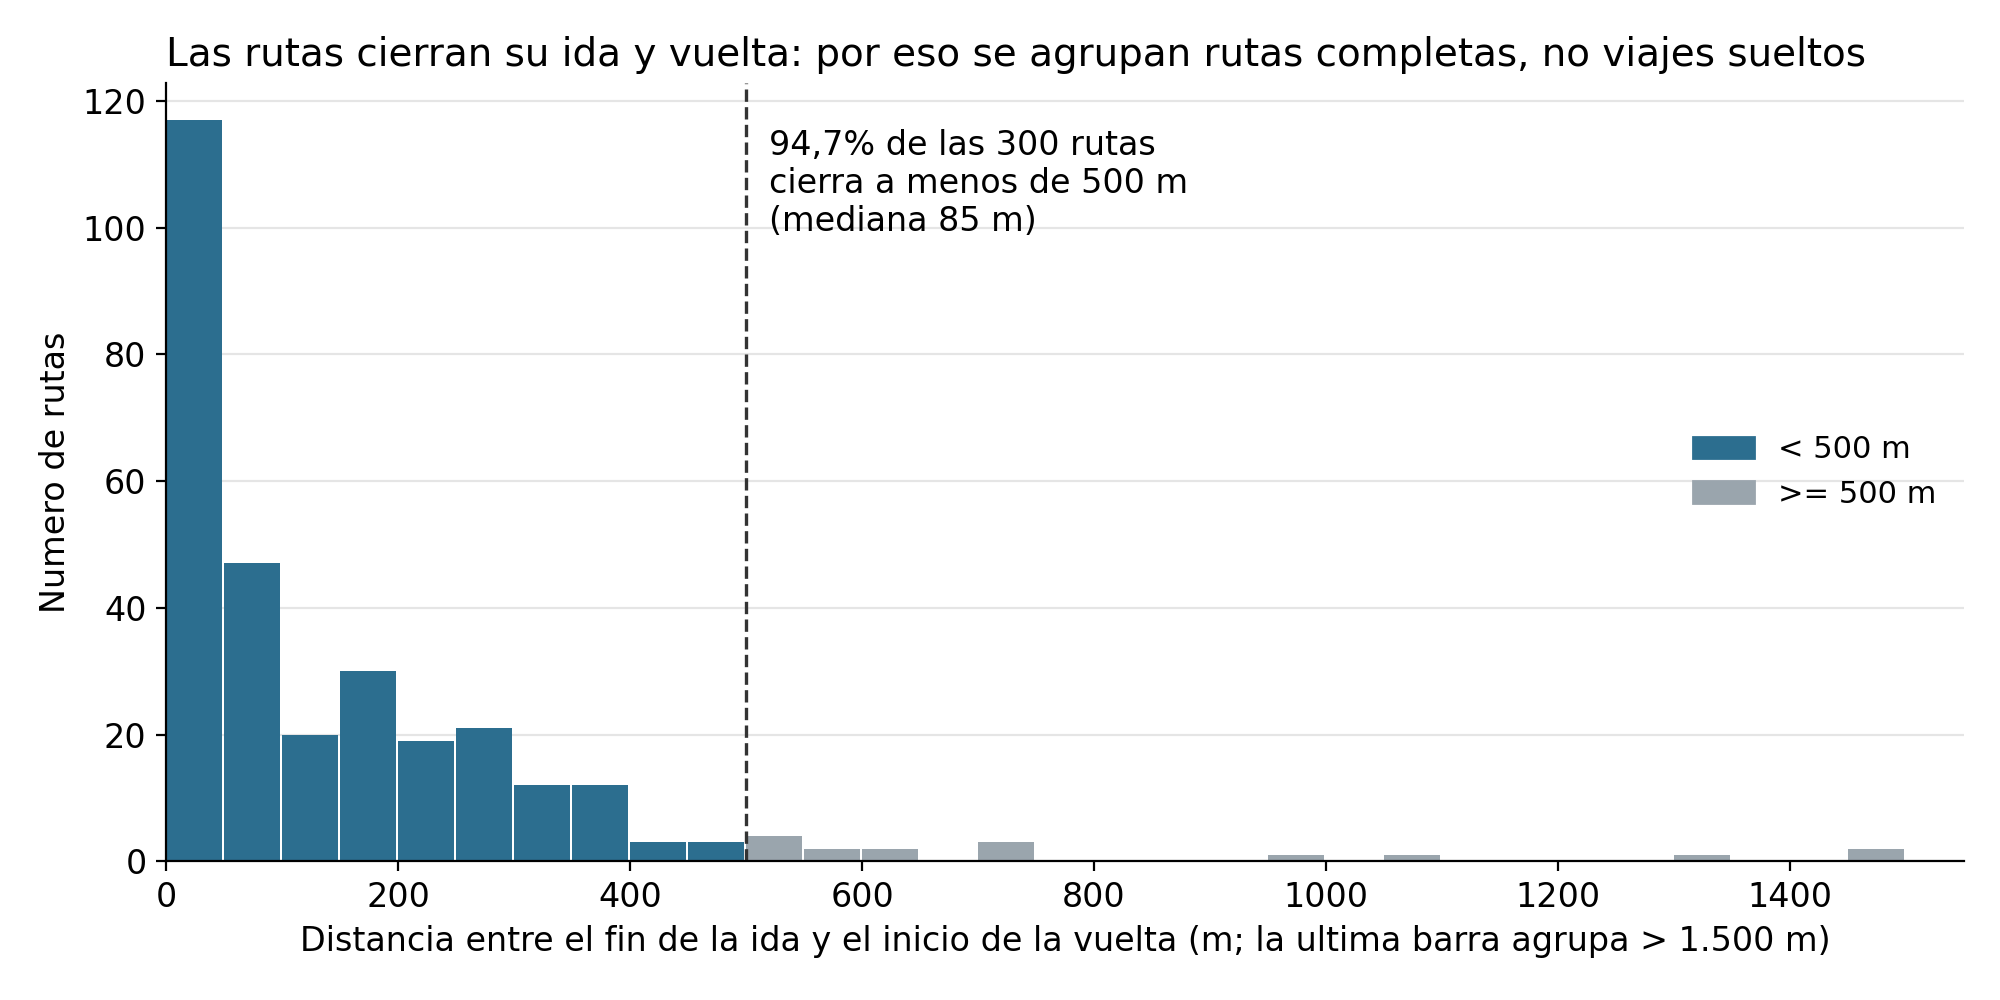
\includegraphics[width=\textwidth]{figures/G2_ida_vuelta.png}
\caption{Distancia entre el término de la ida y el inicio de la vuelta}
\label{fig:ida-vuelta}
\end{figure}

Ida y vuelta forman entonces un ciclo natural, lo que respalda agrupar las rutas completas, por ejemplo al asignarlas a un electroterminal, y no cada viaje por separado.

Por otro lado, se unio el electroterminal de Los Espinos con el de Santa Rosa, que distan de 1,1 Km, nada en comparacion al resto que estan entre 12 a 18 km de estos. Esta union se debe a que al evaluar el caso base con ambos separados, Los Espinos resulta infactible, porque la energía que debe reponer equivale entre 102,6\% y 104,0\% de la que sus puestos pueden entregar en un día. Unido a Santa Rosa, ese porcentaje baja a 82,5\% y el déficit desaparece. Por esta razón, los dos se tratan como un solo electroterminal de 270 puestos.

Por último, los datos presentan limitaciones que conviene tener presentes al interpretar los resultados. En primer lugar, la oferta programada por RED hace de demanda, de modo que el plan debe cubrir todas las expediciones, incluso aquellas que en la práctica irían con pocos pasajeros. A esto se suma que todos las expediciones de un mismo patron de viajes, tienen igual consumo energetico, por lo que no se consideran la congestión, la topografía ni la variabilidad de la operación real. En consecuencia, en horas punta los viajes reales serían más lentos, y los encadenamientos posibles entre viajes resultan algo optimistas. 

\section{Supuestos}
\label{sec:supuestos-informe2}

Para el desarrollo de la metodología, fue necesario definir una serie de supuestos. Cada uno se presenta con sus respectivas justificaciones, sus límites y el análisis de sensibilidad realizado o planificado para la próxima entrega.

\textbf{2.4.1. Factor de desvío de deadhead}

Todo desplazamiento sin pasajeros (deadheads) se calcula como la distancia en línea recta multiplicada por 1,3, a una velocidad de 20 km/h. No se utiliza la red vial de OpenStreetMap.

Usar distancia euclidiana es una decisión de modelación del grupo, pero que probablemente puede ser criticada. Por eso se respaldó el factor con datos propios: en los 839 trazados GTFS se revisaron los puntos separados por rangos de [1-3 km]y [3-5 km] de recorrido, para el interlining y los pullout/pullin respectivamente, y se comparó su distancia real con su distancia en línea recta. 

    \begin{center}
    \begin{tabular}{|p{4.3cm}|p{3cm}|p{4cm}|}
    \hline
    Tipo de desplazamiento & Escala & Factor real (mediana) \\
    \hline
    Interlining & 1-3 km & 1,04 - 1,22 \\
    \hline
    Pullout/pullin & 5-15 km & 1,29 - 1,38 \\
    \hline
    \end{tabular}
    \end{center}

Se concluye que en el caso del interlining el factor de 1,3 es conservador, ya que queda sobre la mediana. Mientras que en desplazamientos de pullout/pullin, el factor queda cercano a la mediana medida, pero podría subestimar levemente la distancia a escalas largas.

Para el análisis de sensibilidad, sobre el escenario E1, variar el factor entre 1,2 y 1,5 mueve la flota entre -1\% y +1\%. Usar el valor medido (1,3) aumenta el costo de operación en 0,6\%. El factor afecta principalmente el costo de los kilómetros vacíos y no la factibilidad del interlining, que ocurre a distancias cortas donde el factor de 1,3 es más acertado. La sensibilidad a la velocidad (15 y 25 km/h) está planificada y queda pendiente de ejecución.

\textbf{2.4.2 Radio máximo de interlining}

Solo se permite encadenar viajes de rutas distintas cuando la distancia de desplazamiento entre ellos es menor o igual a 3 km. Este valor se compara contra la distancia ya multiplicada por 1,3, por lo que equivale a unos 2,3 km en línea recta, es decir, unos 9 minutos de traslado a 20 km/h. 
El radio es una decisión de tamaño del modelo: sin un límite habría que considerar casi todos los pares de viajes, del orden de miles de millones de arcos. No responde a una medición.

\begin{center}
    \begin{tabular}{|p{3.2cm}|p{3.2cm}|p{3.2cm}|p{3.2cm}|}
    \hline
    Radio de interlining & Cantidad de buses & Variación de flota & Tiempo de ejecución \\
    \hline
    1 km & 8.198 & +11,3\% & \textasciitilde20 s \\
    \hline
    2 km & 7.577 & +2,9\% & \\
    \hline
    3 km & 7.366 & & \\
    \hline
    4 km & 7.201 & -2,2\% & \\
    \hline
    5 km & 7.118 & -3,4\% & \textasciitilde120 s \\
    \hline
    \end{tabular}
    \end{center}

Respecto del caso base, el costo de operación aumenta un 11,0\% con un radio de 1 km y disminuye un 3,3\% con uno de 5 km. La reducción de flota presenta rendimientos decrecientes: cada kilómetro adicional permite reducirla menos que el anterior.

Se mantiene 3 km en el caso base, porque ampliarlo exigiría rehacer la etapa de carga con jornadas más largas. Elegir el radio por costo total incluyendo la carga queda como trabajo para la entrega final. 

\textbf{2.4.3. Nivel de carga cíclico}

Todo bus inicia y termina el día con el mismo nivel de batería L, que además es el tope de carga. Se considera L = 100\%, y los ciclos que la carga no alcanza a cerrar se cubren con buses de reserva.

El nivel no se fijó por criterio propio. Se realizó un barrido de ocho niveles (100\%, 90\%, 80\%, 70\%, 65\%, 60\%, 55\% y 50\%) y se eligió el de menor costo total entre las soluciones factibles, entendiendo la condición cíclica como una restricción y no como un indicador. En E1 y E0, el menor costo total corresponde a 100\%. Ningún nivel entre 100\% y 55\% cumple el ciclo sin reservas con la política de carga reactiva. 


\section{Indicadores de desempeño (KPIs)}
\label{sec:kpis-informe2}
 Los indicadores se definieron para responder a una decisión concreta del problema. Cada uno se obtiene para todos los escenarios de la escalera,permitiendo aislar el efecto de cada decisión individualmente al comparar escenarios consecutivos.

\begin{center}
    \begin{tabular}{|p{1cm}|p{5cm}|p{5cm}|p{5cm}|}
    \hline
     & KPI & Definición & Desición que evalua \\
    \hline
    1 & Costo total (USD/día) & Flota + reservas + km vacíos + espera + energía + eventos de carga. & Todas (es el objetivo)\\
    \hline
    2 & Número de buses & Flota operativa + buses de reserva & 	Asignación y clustering \\
    \hline
    3 & \% km de deadheading & 	km sin pasajeros / km totales & Encadenamiento y clustering\\
    \hline
    4 & Costo medio de la energía & USD/kWh cargado (+ \% de la energía cargada en valle) & Programación de carga \\
    \hline
    \end{tabular}
    \end{center}


\chapter[DISCUSI\'ON METODOL\'OGICA]{Discusi\'on metodol\'ogica}
\section{Revisión bibliográfica de la metodología}
 
En la literatura de buses eléctricos se distinguen dos enfoques: los modelos integrados, que deciden al mismo tiempo qué viajes hace cada bus y cuándo carga, y los enfoques secuenciales, que separan estas decisiones en etapas \cite{perumal2022}. Los integrados entregan mejores soluciones, pero se han aplicado a instancias mucho más chicas que la nuestra y por lo general se resuelven con heurísticas como ALNS \cite{wen2016, wang2024}. Dado el tamaño del caso, con 64.502 expediciones diarias, optamos por una descomposición secuencial en cuatro etapas: asignar las rutas a electroterminales, construir las jornadas sin considerar la batería, cortarlas y reencadenarlas según la batería, y programar la carga en cada electroterminal.

La principal fortaleza de este enfoque es que casi todas sus etapas se resuelven de forma exacta y en poco tiempo. Tanto la construcción de jornadas como su reencadenamiento usan la red espacio-tiempo de \citeA{kliewer2006}, pensada para problemas con varios depósitos y muchos viajes, cuya relajación lineal entrega directamente soluciones enteras. Además, cada etapa tiene una referencia con la cual comparar, lo que permite medir cuánto se pierde al dividir el problema. Por ejemplo, agrupar las rutas por electroterminal solo agrega 311 buses, algo que una heurística como ALNS no permitiría cuantificar. El MILP se reserva para la programación de la carga, que es donde se cruzan el horario, la tarifa y los puestos disponibles, en línea con \citeA{zhang2024} y \citeA{zhou2024}. Por último, como cada electroterminal es un problema independiente, la propuesta se pudo probar en un terminal completo, La Reina, donde reduce la flota total en cerca de un 30\% frente a la carga reactiva.
 
La debilidad más importante sigue siendo que la construcción de jornadas no considera la batería, que es el costo típico de los enfoques secuenciales \cite{perumal2022}. La tercera etapa corrige esto después, cortando y reencadenando las jornadas, pero no las rediseña desde cero, por lo que la flota final sigue siendo mayor que la de las jornadas sin batería. Además, las etapas 3 y 4 no se retroalimentan: la tercera no ve los puestos de carga, y la única forma de anticipar las colas es dejar una holgura antes de que cada bus vuelva a salir, lo que no elimina los buses de reserva. En la programación de la carga también hay que elegir entre precisión y tiempo de cálculo. El modelo agregado se resuelve rápido, pero en algunos minutos del día supera los puestos disponibles, mientras que el modelo detallado respeta mejor la capacidad y no alcanza a resolverse en un tiempo razonable. Hasta ahora, todo esto solo se ha probado en La Reina, y los terminales más grandes quedan para la entrega final.
 
Respecto a los supuestos, el más discutible es la carga lineal. \citeA{olsen2020} muestran que este supuesto subestima el tiempo real de carga, porque la carga se vuelve más lenta cerca del 100\%, y que puede generar jornadas imposibles de cumplir. Como en nuestro caso la carga ya es el cuello de botella, los resultados de energía probablemente son optimistas. Además, la tercera etapa supone que cada bus se recarga completo entre tramos, y el consumo se considera constante, sin considerar la pendiente ni la congestión. En cambio, el tamaño de los bloques de tiempo del MILP resultó poco relevante para los resultados. Para la entrega final, las mejoras prioritarias son llevar las etapas 3 y 4 a toda la red y coordinarlas entre sí. Si esto no basta, la alternativa natural es una heurística integrada como la de \citeA{wen2016}.

\section{Metodología}

La metodologia organiza la asignacion de expediciones a buses y la planificacion de sus recargas mediante una secuencia de etapas. A partir de recorridos y horarios previamente definidos, busca reducir el costo operativo mediante el uso compartido de buses entre rutas
(\textit{interlining}) y la programación anticipada de la carga, considerando la autonomía de los vehículos y la infraestructura disponible. 




\subsection{Asignación de rutas a electroterminales}

La primera etapa determina el electroterminal desde el cual operará cada
ruta. Para ello, se considera la distancia a los paraderos donde comienzan
y terminan sus expediciones, ponderada por la frecuencia con que se utilizan estos paraderos.

Sea $R$ el conjunto de rutas y $D$ el conjunto de electroterminales
disponibles. Para cada ruta $r \in R$, se define $T_r$ como el conjunto
de paraderos donde comienzan o terminan sus expediciones. El parámetro
$\ell(k,d)$ representa la distancia estimada entre el paradero
$k \in T_r$ y el electroterminal $d \in D$.

Asimismo, $w_{rk}$ representa el peso relativo del paradero $k$, según
la frecuencia con que aparece como origen o destino de las expediciones
de la ruta $r$. Estos pesos satisfacen:

\begin{equation}
    w_{rk} \geq 0
    \qquad \forall r \in R,\; k \in T_r.
\end{equation}

\begin{equation}
    \sum_{k \in T_r} w_{rk} = 1
    \qquad \forall r \in R.
\end{equation}

Cada ruta se asigna al electroterminal que minimiza la distancia promedio
ponderada a sus paraderos terminales:

\begin{equation}
    d(r) \in
    \operatorname*{arg\,min}_{d \in D}
    \sum_{k \in T_r} w_{rk}\,\ell(k,d)
    \qquad \forall r \in R.
\end{equation}

La expresión $\operatorname*{arg\,min}$ identifica el electroterminal
que alcanza la menor distancia ponderada. Si varios electroterminales
presentan el mismo valor mínimo, se selecciona uno de ellos.

Este procedimiento entrega una asignación única por ruta y forma grupos
de rutas asociados a cada electroterminal. La asignación obtenida se
mantiene fija durante la construcción de jornadas y las etapas posteriores
de carga. Por lo tanto, constituye un dato de entrada para esas etapas
y solo requiere recalcularse si cambian los datos o el criterio de asignación.

\subsection{Construcción de jornadas con interlining}

Una jornada corresponde a una secuencia de expediciones atendidas por
un bus, desde su salida del electroterminal hasta su regreso. En esta
etapa se determina qué expediciones pueden realizarse consecutivamente
y cuántos buses se necesitan, considerando los costos de utilización
de flota, desplazamientos sin pasajeros y espera.

Se permite el \textit{interlining}, de modo que un mismo bus puede atender
expediciones de distintas rutas durante su jornada, siempre que
pertenezcan al mismo electroterminal y que sus conexiones sean compatibles
en tiempo y distancia. Esto permite aprovechar oportunidades de conexión
entre rutas y reducir tiempos ociosos y necesidades de flota.

\paragraph{Compatibilidad entre expediciones.}

Sea $V$ el conjunto de expediciones y $U$ el conjunto de nodos de eventos
que representan oportunidades de conexión y espera. Cada expedición
$i \in V$ tiene una ruta $r_i$, una hora de salida $s_i$ y una hora
de llegada $f_i$.

La distancia y el tiempo de traslado vacío entre el destino de la
expedición $i$ y el origen de la expedición $j$ se denotan por
$\ell_{ij}$ y $\tau_{ij}$, respectivamente. El parámetro $\delta$
representa el tiempo mínimo de preparación entre expediciones, mientras
que $R_{\max}$ corresponde a la distancia máxima permitida para conectarlas.

Para conectar una expedición $i$ con una expedición $j$, se consideran
sus rutas $r_i$ y $r_j$ y los electroterminales asignados a ellas,
$d(r_i)$ y $d(r_j)$. Se denota por $f_i$ la hora de término de $i$
y por $s_j$ la hora de inicio de $j$. El traslado vacío desde el
destino de $i$ hasta el origen de $j$ tiene una distancia
$\ell_{ij}$ y una duración $\tau_{ij}$. Además, $\delta$ es el
tiempo mínimo de preparación y $R_{\max}$ la distancia máxima
permitida para la conexión. 
Una expedición $i$ puede conectarse con una expedición $j$ cuando
se cumplen las siguientes condiciones:

\begin{equation}
    \begin{aligned}
        d(r_i) &= d(r_j), \\
        f_i + \tau_{ij} + \delta &\leq s_j, \\
        \ell_{ij} &\leq R_{\max}.
    \end{aligned}
\end{equation}

La primera condición exige que las rutas de ambas expediciones
pertenezcan al mismo electroterminal. A diferencia del caso base,
no se exige que $r_i = r_j$, por lo que se admiten conexiones entre
rutas diferentes.

La segunda condición garantiza que el bus termine la expedición $i$
y disponga de tiempo suficiente para trasladarse al origen de $j$
y completar la preparación mínima antes de su salida. La tercera
limita la distancia del desplazamiento sin pasajeros. Solo se incorporan
a la red las conexiones que cumplen estas condiciones.

\paragraph{Representación mediante una red de flujo.}

La construcción de jornadas se representa mediante una red cuyos arcos
describen las actividades disponibles para los buses. El conjunto de
arcos $A$ se compone de cinco tipos:

\begin{itemize}
    \item $A_{\mathrm{out}}$: salidas del electroterminal hacia una
    primera expedición.

    \item $A_{\mathrm{dh}}$: traslados vacíos entre el final de una
    expedición y un paradero de salida.

    \item $A_{\mathrm{wait}}$: espera entre eventos consecutivos.

    \item $A_{\mathrm{start}}$: acceso desde un evento a una expedición.

    \item $A_{\mathrm{in}}$: regreso al electroterminal al finalizar
    una jornada.
\end{itemize}

Las líneas de tiempo se organizan por paradero y electroterminal,
permitiendo conexiones entre las rutas del mismo grupo. Los arcos
de salida y regreso se vinculan al electroterminal correspondiente,
de manera que cada jornada comience y termine en su electroterminal base.

\paragraph{Variable de decisión.}

Para cada arco $a \in A$, se define $x_a$ como la cantidad de buses
que utilizan dicho arco:

\begin{equation}
    x_a \geq 0
    \qquad \forall a \in A.
\end{equation}

La formulación conserva una estructura de flujo de red con requerimientos
enteros, lo que permite obtener una solución óptima entera mediante
programación lineal. El número de buses utilizados corresponde al flujo
total de salida de los electroterminales:

\begin{equation}
    B = \sum_{a \in A_{\mathrm{out}}} x_a.
\end{equation}

\paragraph{Función objetivo.}

Se minimiza la suma del costo fijo de los buses, el costo de los kilómetros
recorridos sin pasajeros y el costo de espera:

\begin{equation}
    \min\;
    \sum_{a \in A_{\mathrm{out}}}
    \left(c_B + c_D \ell_a\right)x_a
    +
    \sum_{a \in A_{\mathrm{dh}} \cup A_{\mathrm{in}}}
    c_D \ell_a x_a
    +
    \sum_{a \in A_{\mathrm{wait}}}
    c_W t_a x_a.
\end{equation}

Aquí, $c_B$ es el costo por bus utilizado, $c_D$ el costo por kilómetro
vacío y $c_W$ el costo por minuto de espera. Los parámetros $\ell_a$
y $t_a$ representan la distancia y el tiempo de espera asociados al arco.

El primer término considera la activación del bus y su traslado desde
el electroterminal hacia la primera expedición. El segundo incorpora
los traslados vacíos entre expediciones y el regreso al electroterminal.
El tercero contabiliza las esperas entre viajes.

El costo de los kilómetros comerciales se omite de esta función objetivo,
puesto que todas las expediciones deben realizarse y ese componente
permanece constante entre soluciones. Los costos energéticos y de recarga
se incorporan en etapas posteriores.

\paragraph{Restricciones.}

Denotando por $\delta^{-}(n)$ y $\delta^{+}(n)$ los conjuntos de arcos
que entran y salen del nodo $n$, respectivamente, cada expedición debe
recibir y entregar exactamente un bus:

\begin{equation}
    \sum_{a \in \delta^{-}(i)} x_a = 1
    \qquad \forall i \in V.
\end{equation}

\begin{equation}
    \sum_{a \in \delta^{+}(i)} x_a = 1
    \qquad \forall i \in V.
\end{equation}

Estas restricciones aseguran que cada expedición se atienda una sola vez.
En los nodos de eventos se exige conservación de flujo:

\begin{equation}
    \sum_{a \in \delta^{-}(u)} x_a
    =
    \sum_{a \in \delta^{+}(u)} x_a
    \qquad \forall u \in U.
\end{equation}

Así, los buses que ingresan a un evento deben continuar mediante alguna
actividad permitida. La construcción temporal de la red y sus conexiones
de salida y regreso permiten formar jornadas que parten y terminan
en el electroterminal correspondiente.

El resultado de esta etapa es el número inicial de buses y la secuencia
de expediciones de cada jornada, incluyendo sus traslados y esperas.
Estas jornadas cumplen las condiciones de cobertura y compatibilidad
temporal, pero su factibilidad energética deberá evaluarse en las
etapas posteriores de la metodología.

\section{Caso base}

\subsection{Propósito y criterio de construcción}

El caso base, denominado E0, representa una operación organizada por ruta,
sin \textit{interlining} y con una política de carga reactiva. Cada bus
atiende exclusivamente expediciones de una misma ruta y las decisiones
de recarga responden a sus necesidades inmediatas de energía. Esta
configuración permite establecer una referencia para evaluar el efecto
de habilitar conexiones entre rutas y programar anticipadamente las recargas.

Su construcción combina un modelo de optimización que asigna expediciones
a buses, inicialmente sin restricciones de batería, y una simulación que
incorpora posteriormente los requerimientos energéticos. Por lo tanto,
el caso base optimiza la construcción de jornadas dentro de cada ruta pero sin permitir interlining, y ademas no coordina anticipadamente la asignación de viajes con la carga.

Se utilizan las mismas expediciones, horarios, parámetros de costos
y condiciones de infraestructura que en los escenarios de mejora.
La flota es irrestricta, ademas se mantiene la representación conjunta de Los Espinos y Santa Rosa
como un electroterminal operativo con capacidad de carga compartida.

\subsection{Asignación de rutas y construcción de jornadas}

La asignación de rutas a electroterminales utiliza el procedimiento
descrito en la primera etapa de la metodología. Cada ruta se asigna
al electroterminal que minimiza la distancia promedio ponderada a sus
paraderos de inicio y término. Esta asignación se calcula previamente
y permanece fija durante la construcción de jornadas y la simulación
de carga.

La construcción de jornadas mantiene las variables, la función objetivo
y las restricciones de cobertura y conservación de flujo presentadas
en la segunda etapa de la metodología. La diferencia es que solo se
permiten conexiones entre expediciones de una misma ruta. Para conectar
las expediciones $i$ y $j$, se añade la condición:

\begin{equation}
    r_i = r_j.
\end{equation}

Esta condición restringe el conjunto de conexiones disponibles e impide
el \textit{interlining}. En consecuencia, las líneas de tiempo se organizan
por paradero y ruta, manteniendo las condiciones de compatibilidad
temporal, distancia máxima de traslado y retorno al electroterminal.
El resultado es un conjunto inicial de jornadas que cubre todas las
expediciones, cuya factibilidad energética se revisa en la siguiente etapa.

\subsection{Incorporación de carga reactiva}

Las jornadas iniciales se evalúan mediante una simulación que actualiza
la energía disponible de cada bus después de cada expedición y traslado
sin pasajeros. El bus comienza con el nivel de batería definido para
el caso base, correspondiente al 100\%, y debe conservar en todo momento
al menos el 10\% de su capacidad.

Sea $Q_i$ la energía disponible al terminar la expedición $i$.
Si la siguiente expedición asignada es $j$, el bus continúa cuando
se cumple:

\begin{equation}
    Q_i - E_{ij} - E_j - E_{jd} \geq Q_{\min},
\end{equation}

donde $E_{ij}$ es la energía requerida para trasladarse desde el final
de $i$ al inicio de $j$, $E_j$ es el consumo de la expedición $j$,
$E_{jd}$ es la energía necesaria para regresar desde su término
al electroterminal y $Q_{\min}$ es el nivel mínimo de energía permitido.
Esta condición verifica que el bus pueda realizar la siguiente expedición
y regresar al electroterminal sin bajar del mínimo de batería.

Si la condición no se cumple, el bus intenta regresar al electroterminal
y recargar antes de la siguiente expedición. Para determinar si esto
es posible, se consideran los tiempos de traslado, la disponibilidad
de un puesto de carga y el tiempo necesario para recibir la energía
requerida. Se admite una carga parcial cuando permite continuar
la operación, respetando el horario de salida de la siguiente expedición.

Cuando no existe tiempo suficiente para realizar la recarga y llegar
a la siguiente salida, la jornada se divide y un nuevo bus atiende
las expediciones restantes. Así, la flota obtenida después de incorporar
las restricciones energéticas puede superar la calculada inicialmente
por el modelo de asignación.

La simulación también incorpora la recarga final necesaria para recuperar
el nivel de batería de partida y repetir la operación al día siguiente.
Si un bus no termina de cargar antes de su próxima salida, se contabiliza
un bus de reserva ya cargado para cubrirla, mientras el primero completa
su recarga. Tanto la energía repuesta como el costo de las reservas
se incluyen en la evaluación. Esta representación supone una rotación
de buses entre días; las reservas no sustituyen la energía que debe
recargarse ni aumentan la capacidad de los cargadores.

La política es reactiva porque decide cargar según la necesidad inmediata
del bus, sin anticipar oportunidades futuras ni seleccionar horarios
en función de las tarifas eléctricas. Esto permite evaluar posteriormente
el beneficio de introducir una programación de carga.

\subsection{Evaluación y validación del caso base}

El caso base constituye una referencia adecuada porque utiliza reglas
operacionales claras, como mantener los buses dentro de una misma ruta y recargar
cuando la energía resulta insuficiente para continuar. Representa una
alternativa de planificación reproducible, sin asumir que reproduce
exactamente la operación real de RED. Al mantener las mismas condiciones
de demanda, infraestructura y costos que los escenarios de mejora, permite
atribuir las diferencias observadas a las decisiones que se modifican.

La evaluación se realiza sobre el día laboral completo, compuesto por
64.502 expediciones y 417 rutas, después de pruebas iniciales sobre
subconjuntos de rutas. La asignación a electroterminales permanece fija
y las jornadas obtenidas alimentan la simulación energética.

La verificación comprueba que cada expedición se cubra exactamente una vez,
que las conexiones respeten los horarios y tiempos de traslado, que cada
jornada atienda una sola ruta y que los buses regresen a su electroterminal.
Para comprobar la cobertura se utilizan identificadores únicos por
expedición, distinguiendo las distintas salidas de un mismo patrón de viaje.

En términos energéticos, se revisan el nivel mínimo de batería, la capacidad
simultánea de los cargadores y la reposición de la energía consumida.
Se distinguen los buses adicionales por división de jornadas de las reservas
necesarias cuando la recarga final supera la siguiente salida. Bajo la
rotación adoptada, se exige ausencia de déficit energético y atrasos de
carga inferiores a 24 horas: las reservas cubren demoras, pero no resuelven
una insuficiencia de infraestructura.

El desempeño se mide mediante los KPIs definidos, incluyendo costo total
y desglose, flota requerida, kilómetros sin pasajeros y utilización de
cargadores. La flota inicial, los buses adicionales y las reservas se reportan
por separado para identificar el efecto de las restricciones energéticas.

Finalmente, la comparación con E1 mantiene la carga reactiva y habilita
únicamente el \textit{interlining}. La carga optimizada se evalúa sobre
instancias con las mismas jornadas y capacidades para ambas políticas.
Los resultados se presentan en la sección de resultados y análisis,
distinguiendo entre la red completa y las instancias reducidas.

\chapter[TRABAJO Y RESULTADOS PRELIMINARES]{Trabajo desarrollado y resultados preliminares}
\section{Implementación y herramientas}
\textit{[Documentar herramientas, lenguajes, solver y estructura del código.
Indicar dónde se compartirán los códigos (por ejemplo, enlace al repositorio o
archivo adjunto) y cómo reproducir los experimentos.]}

\section{Prueba de concepto o prototipo}
\textit{[Describir la instancia de prueba, las simplificaciones y su
justificación, los supuestos, el diseño del experimento y cómo se verificó la
implementación.]}

\section{Resultados preliminares}
\textit{[Presentar resultados con tablas y figuras legibles. Reportar la
variabilidad entre corridas o escenarios cuando corresponda.]}

\section{Resultados del caso base}

El caso base (E0) representa la operación sin optimizar: cada ruta usa solo sus propios buses, opera desde el electroterminal más cercano y carga de forma reactiva, es decir, solo cuando la batería no le alcanza para el siguiente viaje y sin considerar la tarifa. Los electroterminales Los Espinos y Santa Rosa, ubicados a 1,1 km de distancia, se modelan como un solo terminal de 270 puestos, porque al tratarlos por separado Los Espinos no tiene capacidad de carga suficiente y el caso base resulta infactible. Para aislar el efecto del \textit{interlining}, se evaluó también un escenario E1, que es igual a E0 pero permite combinar viajes de distintas rutas dentro de un mismo electroterminal. En ambos escenarios, cada bus debe terminar el día con la batería al 100\%. Cuando esto no se logra, se agrega un bus de reserva.

E0 tiene un costo de 3.958.063 USD/día, mientras que E1 llega a 3.751.250 USD/día, un 5,2\% menos. Sin considerar la batería, el \textit{interlining} reduce la flota de 8.654 a 7.366 buses ($-$14,9\%). Sin embargo, al incluir la carga, esta ventaja se reduce a 745 buses ($-$5,6\%). Esto ocurre porque, en E1, las jornadas son más largas y requieren más energía, por lo que hay que dividir más jornadas y agregar más buses de reserva (2.207 en E1, frente a 1.988 en E0). El principal resultado es que la batería es el cuello de botella: al incluir la carga, la flota sube un 53\% en E0 (a 13.247 buses) y un 70\% en E1 (a 12.502 buses) respecto de la asignación de buses sin considerar la batería. Además, todos los electroterminales llegan al 100\% de ocupación en algún momento del día.

Respecto a los KPIs, el número de buses y el porcentaje de km sin pasajeros sí distinguen entre ambos escenarios. En cambio, el costo medio de la energía (0,14 USD/kWh) y el porcentaje cargado en horario valle (cerca del 50\%) son prácticamente iguales, porque los dos escenarios cargan de forma reactiva. Por lo tanto, estos últimos indicadores solo serán útiles para evaluar la programación de la carga, y proponemos agregar el número de buses de reserva como KPI, ya que es el que mejor refleja el costo de no planificar la carga.

\section{Discusión}
\textit{[Explicar qué se aprendió del prototipo, sus límites y cómo los
resultados orientan la implementación final.]}

\chapter[CONCLUSIONES]{Conclusiones}
\textit{[Sintetizar los aprendizajes y resultados principales; evaluar la
robustez, fortalezas y limitaciones del enfoque; indicar implicancias prácticas
y proponer mejoras concretas hacia la entrega final. No introducir resultados
que no se hayan presentado antes.]}

\chapter[PASOS FUTUROS]{Pasos futuros}
\section{Avance respecto del plan del Informe 1}
\textit{[Indicar qué actividades se cumplieron, cuáles se retrasaron o cambiaron,
y explicar las dificultades y ajustes de rumbo.]}

\section{Plan de trabajo actualizado}

Habiendo implementado el caso base y evaluado preliminarmente la metodología
de descomposición secuencial, el trabajo futuro se concentrará en mejorar la
coordinación entre las jornadas de los buses y sus requerimientos de recarga.
A partir de las limitaciones identificadas, se proponen las siguientes
cinco etapas:

\begin{enumerate}
    \emergencystretch=2em
    \renewcommand{\labelenumi}{(\roman{enumi})}

    \item \textbf{Mejorar la generación de ventanas de carga.}
    Se evaluará incorporar los requerimientos de batería durante la
    construcción o ajuste de las jornadas, considerando los tiempos
    necesarios para trasladarse al electroterminal y recargar.
    Actualmente, estas oportunidades se determinan mediante una política
    reactiva, lo que puede obligar a dividir jornadas y utilizar buses
    adicionales. Se estudiará una formulación de optimización que permita
    seleccionar ventanas de carga compatibles con los viajes programados,
    buscando reducir la flota necesaria y manteniendo la cobertura de
    todas las expediciones.

    \item \textbf{Ampliar la implementación del MILP de carga.}
    Se extenderán progresivamente las pruebas realizadas en instancias
    reducidas de Los Espinos--Santa Rosa hacia conjuntos mayores de buses
    y otros electroterminales. En cada ejecución se registrarán los tiempos
    de resolución y las brechas de optimalidad, para determinar la escala
    que puede abordarse con los recursos disponibles. Si se presentan
    dificultades computacionales, se evaluarán mejoras de la formulación
    y estrategias de resolución por electroterminal, con el objetivo de
    avanzar hacia la programación de carga de toda la red.

    \item \textbf{Validar y ajustar los supuestos del modelo.}
    Se profundizará el análisis de sensibilidad de las distancias y
    velocidades de los traslados sin pasajeros, los tiempos mínimos entre
    viajes y el radio permitido para el \textit{interlining}. También se
    compararán distintas duraciones de los intervalos del MILP, para
    evaluar cómo la discretización temporal afecta los costos, las
    reservas y el tiempo de cálculo. Estas pruebas permitirán justificar
    mejor las simplificaciones adoptadas y determinar cuáles requieren
    ajustes antes de consolidar la solución final.

    \item \textbf{Evaluar la metodología bajo distintos tipos de día.}
    Una vez validado el funcionamiento para el día laboral, se buscará
    extender el análisis a sábados y domingos, sujeto al tiempo disponible.
    Para ello, se prepararán las expediciones correspondientes a cada tipo
    de día y se ejecutará nuevamente la metodología, considerando sus
    diferencias de horarios y frecuencias. En todos los casos se verificará
    la cobertura de los viajes, la factibilidad de los traslados, los límites
    de batería y la capacidad de carga de los electroterminales.

    \item \textbf{Analizar los resultados y preparar los entregables finales.}
    Se compararán las soluciones obtenidas con el caso base mediante los
    indicadores definidos, distinguiendo el costo total, la flota
    operacional, los buses de reserva y la utilización de los cargadores.
    Se identificarán los beneficios y las limitaciones de cada mejora,
    diferenciando los resultados de instancias reducidas de aquellos
    obtenidos para la red completa. Finalmente, se consolidarán las
    jornadas por bus, los itinerarios de recarga y el desglose de costos,
    junto con las conclusiones del proyecto y la documentación necesaria
    para reproducir los resultados.

\end{enumerate}

\begin{table}[H]
\centering
\caption{Carta Gantt actualizada para los pasos futuros}
\label{tab:gantt-informe2}
\scriptsize
\resizebox{\textwidth}{!}{%
\begin{tabular}{@{}p{0.29\textwidth}p{0.23\textwidth}p{0.18\textwidth}*{6}{c}@{}}
\toprule
\textbf{Actividad / hito}
& \textbf{Depende de}
& \textbf{Responsable(s)}
& \textbf{S1}
& \textbf{S2}
& \textbf{S3}
& \textbf{S4}
& \textbf{S5}
& \textbf{S6} \\
\midrule

1. Mejorar la generación de ventanas de carga
& Metodología y caso base disponibles
& \textit{[Nombre(s)]}
& X & X & X & $\square$ & $\square$ & $\square$ \\

2. Ampliar la implementación del MILP de carga
& Validación inicial de la actividad 1
& \textit{[Nombre(s)]}
& $\square$ & $\square$ & X & X & X & $\square$ \\

3. Validar y ajustar los supuestos del modelo
& Modelo ejecutable; avances de las actividades 1 y 2
& \textit{[Nombre(s)]}
& $\square$ & X & X & X & X & $\square$ \\

4. Evaluar días sábado y domingo
& Modelo laboral validado en las actividades 2 y 3
& \textit{[Nombre(s)]}
& $\square$ & $\square$ & $\square$ & $\square$ & X & $\square$ \\

5. Analizar resultados y preparar los entregables finales
& Resultados progresivos de las actividades 1--4
& \textit{[Nombre(s)]}
& $\square$ & $\square$ & $\square$ & X & X & X \\

Entrega del informe final: 27 de noviembre
& Cierre de la actividad 5
& \textit{[Nombre(s)]}
& $\square$ & $\square$ & $\square$ & $\square$ & $\square$ & X \\

\bottomrule
\end{tabular}%
}
\end{table}

\cleardoublepage
\phantomsection \label{references}
\bibliographystyle{apacite}
\renewcommand{\bibname}{BIBLIOGRAF\'IA}
\setlength{\bibitemsep}{0.3em}
{\small\singlespacing\bibliography{Thesis}}

\appendix
\newpage
\section[Declaraci\'on de uso de IA]{Declaraci\'on de uso de inteligencia artificial en este informe y presentaci\'on asociada}
\newcommand{\firmaBox}[2]{%
  \begin{minipage}[t]{4.2cm}
    \centering
    \IfFileExists{firmas/#2.png}%
      {\includegraphics[width=3.8cm,height=1.7cm,keepaspectratio]{firmas/#2.png}}%
      {\IfFileExists{firmas/#2.jpg}%
        {\includegraphics[width=3.8cm,height=1.7cm,keepaspectratio]{firmas/#2.jpg}}%
        {\IfFileExists{firmas/#2.jpeg}%
          {\includegraphics[width=3.8cm,height=1.7cm,keepaspectratio]{firmas/#2.jpeg}}%
          {\fbox{\begin{minipage}[c][1.7cm][c]{3.7cm}\centering\footnotesize\textit{(firma pendiente)}\end{minipage}}}%
        }%
      }\\[2pt]
    \rule{3.8cm}{0.4pt}\\[2pt]
    \small #1
  \end{minipage}%
}

\noindent\textbf{Grupo:} 24

\vspace{0.35cm}

\noindent\textbf{¿Hicieron uso de herramientas de IA en este informe y/o
presentación?} \quad Sí: $\square$ \qquad No: $\square$

\vspace{0.35cm}

\noindent\textbf{Marquen los usos que correspondan:}

\begin{itemize}
\setlength{\itemsep}{2pt}
\item[$\square$] Apoyo a la redacción, ortografía o estructura gramatical.
\item[$\square$] Apoyo al análisis de datos e información del problema.
\item[$\square$] Búsqueda o filtro de referencias y literatura.
\item[$\square$] Apoyo al desarrollo del modelo.
\item[$\square$] Apoyo al desarrollo de código computacional.
\item[$\square$] Apoyo al análisis de resultados.
\item[$\square$] Apoyo para construir figuras o diagramas.
\item[$\square$] Apoyo para obtener conclusiones.
\item[$\square$] Otro: \rule{8cm}{0.4pt}
\end{itemize}

\noindent\textbf{Herramientas de IA utilizadas y reflexión breve sobre su
aporte, utilidad y verificación de sus resultados:}

\vspace{0.2cm}
\noindent\rule{\textwidth}{0.4pt}\\[0.7cm]
\noindent\rule{\textwidth}{0.4pt}\\[0.7cm]
\noindent\rule{\textwidth}{0.4pt}

\vspace{0.5cm}

\noindent\textbf{Nombres y firmas de todos los integrantes:}

\vspace{0.3cm}

\begin{center}
\begin{tabular}{ccc}
\firmaBox{Nicol\'as Bennett}{nicolas_bennett} & \firmaBox{Antonio De Frutos}{antonio_defrutos} & \firmaBox{Claudio Hasb\'un}{claudio_hasbun} \\
\firmaBox{Agust\'in Irarr\'azaval}{agustin_irarrazaval} & \firmaBox{Joaqu\'in Jim\'enez}{joaquin_jimenez} & \firmaBox{Alonso Muelas}{alonso_muelas}
\end{tabular}
\end{center}

\end{document}